\begin{figure}[H]
\centering
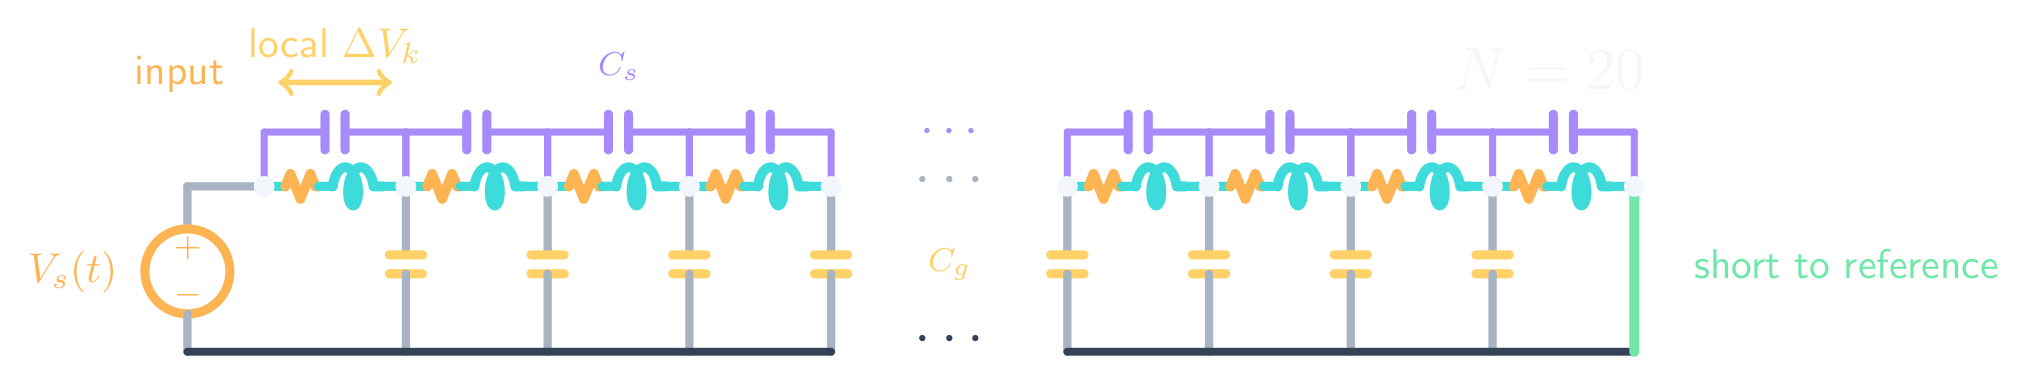
\includegraphics[width=\linewidth]{circuito_grounded.png}
\caption{Escada equivalente do enrolamento. Cada seção tem um ramo série \(R\text{--}L\), uma
capacitância série entre espiras \(\Cs\) (\emph{turn-to-turn}, em roxo, arqueada sobre o ramo) e uma
capacitância shunt para o núcleo aterrado \(\Cg\) (em amarelo). A fonte de surto \(\Vsrc\) entra à
esquerda; o neutro (terminal final) é \emph{solidamente aterrado}. É o mesmo circuito da apresentação
animada e da validação cruzada em ATP.}
\label{fig:circuito-pi}
\end{figure}
